\providecommand{\topdir}{..}
\documentclass[../main.tex]{subfiles}
% \appendtographicspath{./resources/ch1}

\newglossaryentry{P3MEEET}
{
	name=P3MEEET,
	description={A polymer}
}

\begin{document}
    \chapter{Introduction}\label{chap:01-intro}
	
	\section{What is an organic semiconductor?}
	Let's break it down: Organic, and semiconductors.
	If you've done little chemistry before, then organic simply implies it contains carbon. Typically when people think of semiconductors, they think of Si (which is abundant in sand) and gallium-arsenide (GaN) and other sorts of crystalline materials. These alternative materials do not typically contain carbon.
	So what's the interest in carbon? Well carbon is cheap, it's one of the most abundant elements on the earth (see \cref{fig:ch1-elemental_abundance}).
	\begin{figure}[H]
		\centering
		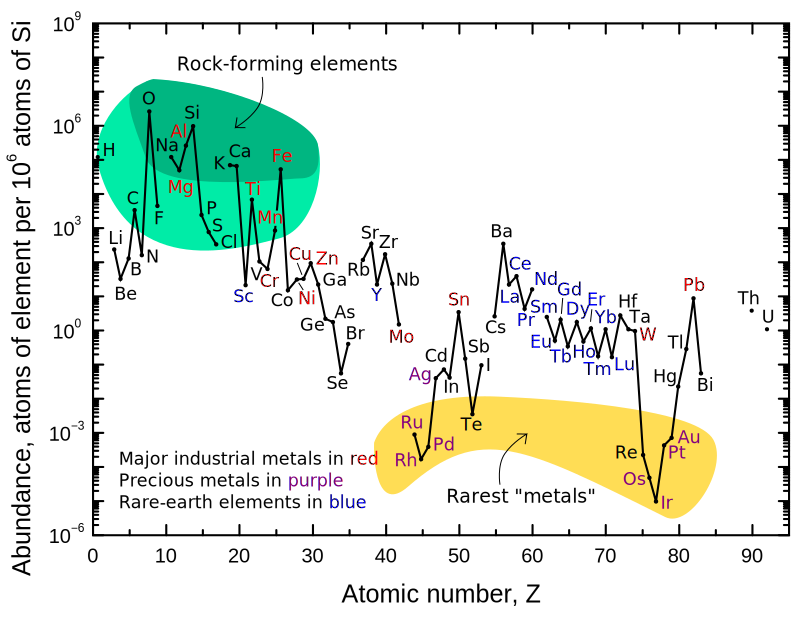
\includegraphics[width=0.5\textwidth]{resources/ch1/elemental-abundances}
		\caption{Elemental abundances, relative to Si, in the earths crust.\autocite{haxel_rare_2005}}
		\label{fig:ch1-elemental_abundance}
	\end{figure}
	
	What about the idea of a semiconductor? A semiconductor is simply a material that has a small bandgap, such providing some energy (such as light) or some potential (such as a voltage) can allow conduction to begin in the material.
	
	Typically, organic semiconductors are polymers molecules, not crystals. However, in smaller polymers cases, such as rubrene\autocite{wang_highly_2023}, crystallisation can occur allowing high quality devices. Mobility compared to their solid-state counterparts is still disadvantageous.

\ifSubfilesClassLoaded{
    \printbibliography{}
    \printglossaries
}{} % we have no 'else' action
    
\end{document}